\section{Validity}
\label{measurement:validity}

This work measured the features executed over repeated, automated interactions
with a website, in a low-trust, unauthenticated browsing scenario.  We treat
these automated measurements as representative of the features that would be
executed when a human visits the website in a similar scenario.

Thus, the work relies on the automated measurement technique
triggering (at least) the browser functionality a human user's browser will
execute when interacting with the same website. This section explains how we
verified this assumption to be reasonable.


\subsection{Internal Validation}
\label{measurement:validity:internal-validation}
\begin{table}[ht]
  \centering
  \begin{tabular}{ l r }
    \toprule
      Round \# &
      Avg. New Standards \\
    \midrule
      2 & 1.56 \\
      3 & 0.40 \\
      4 & 0.29 \\
      5 & 0.00 \\
    \bottomrule
  \end{tabular}
  \caption{Average number of new standards encountered on each subsequent automated crawl of a domain.}
  \label{fig:internal-validation-table}
\end{table}
As discussed in
Section~\ref{measurement:methodology:default-case-measurements}, we applied our
automated measurement technique to each site in the Alexa 10k ten times, five
times in an unmodified browser, and five times with blocking extensions in
place.  We performed five measurements in each condition to with the goal of
capturing the full set of functionality used on the site, since the
measurement's random walk technique means that each subsequent measurement may
encounter different, new parts of the site.

A natural question then is whether five measurements were sufficient to capture
all potentially encountered features per site, or whether additional
measurements would have triggered new standards.  To test this, we examined how
many new standards were encountered on each round of measurement.  If new
standards were still being encountered in the final round of measurement, it
would indicate five measurements were was insufficient to fully measure what
features were used on each site.

\ref{fig:internal-validation-table} shows the results of this verification.
The first column lists each round of measurement, and the second column lists
the number of new standards encountered that had not yet been observed in the
previous rounds (averaged across the entire Alexa 10k).  As the table shows,
the average number of new standards observed on each site decreased with each
measurement, until the fifth measurement for each site, at which point we did
not observe any new features being executed on any site.

From this we concluded that five rounds was sufficient for each domain, and
that further automated measurements of these sites were unlikely to observe new
feature use.


\subsection{External Validation}
\label{measurement:validity:external-validation}
\begin{figure}[h]
  \centering
  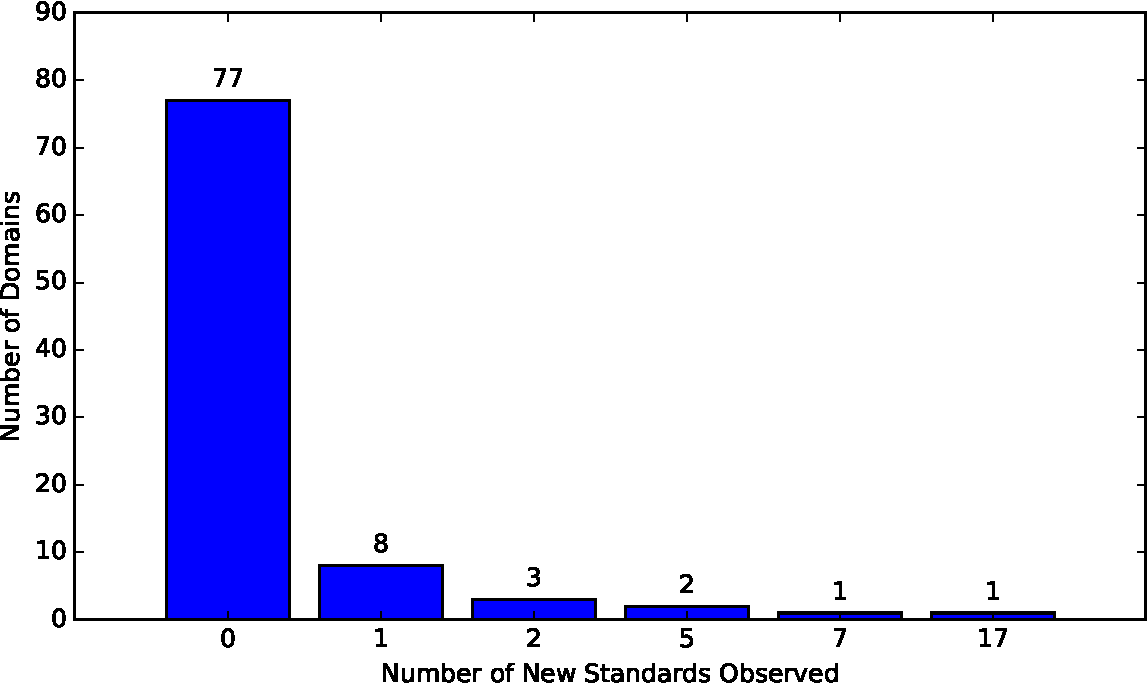
\includegraphics[width=0.5\textwidth]{figures/measurement_external_validation.pdf}
  \caption{Histogram of the number of standards encountered on a domain under manual interaction that were not encountered under automated interaction.}
  \label{fig:external-validation-figure}
\end{figure}

We also tested whether our automated technique observed the same feature
use as human web users.   To do so, we randomly selected 100 sites to visit
from the Alexa 10k and interacted with each for 90 seconds in a casual
web browsing fashion.  This included reading articles and blog posts, scrolling
through websites, browsing site navigation listings, and generally attempting
to exercise what we thought was key functionality on each site.

We interacted with the home page of the site (the page directed to from the raw
domain) for 30 seconds, then clicked on a prominent link we thought a typical
human browser would choose (such as the headline of a featured article) and
interacted with this second page for 30 more seconds.  We then repeated the
process a third time, loading a third page that was interacted with for another
30 seconds.

After omitting pornographic and non-English sites, we completed this process
for 92 different websites. We then compared the features used during manual
interaction with our automated measurements of the same sites.
\ref{fig:external-validation-figure} is a histogram of this
comparison, with the x-axis showing the number of new standards
observed during manual interaction that \textit{were not} observed during
the automated interaction.  As the graph shows, in the majority of cases
(83.7\%), no features were observed during manual interaction that the
automated measurements did not catch.

The graph also shows a few outliers, including a very significant one, where
manual interaction triggered many standards that our automated technique
missed.  On closer inspection, this outlier was due to the site updating its
content between when we performed the automated measurement and the manual
measurement.  The outlier site, \texttt{buzzfeed.com}, is a website that
changes its front page content hour to hour.  The site further features
subsections that are unlike the rest of the site, and can have widely differing
functionality, resulting in very different standard usage over time. We checked
to see if manual evaluation of this site triggered standards not
observed during automated testing on the rest of the Alexa 10k, and did not
find any.

From this we conclude that our automated measurement technique did a generally
accurate job of elicit the feature use a human user would encounter on the web,
even if the technique did not perfectly emulate human feature use in all cases.
